\documentclass{beamer}
\usepackage[utf8]{inputenc}

\usetheme{Boadilla}
\usecolortheme{lily}
\usepackage{amsmath,amssymb,amsfonts,amsthm}
\usepackage{mathtools}
\usepackage{txfonts}
\usepackage{tkz-euclide}
\usepackage{listings}
\usepackage{adjustbox}
\usepackage{array}
\usepackage{tabularx}
\usepackage{lmodern}
\usepackage{circuitikz}
\usepackage{tikz}
\usepackage{graphicx}

\setbeamertemplate{footline}
{
  \leavevmode%
  \hbox{%
  \begin{beamercolorbox}[wd=\paperwidth,ht=2.25ex,dp=1ex,right]{author in head/foot}%
    \insertframenumber{} / \inserttotalframenumber\hspace*{2ex} 
  \end{beamercolorbox}}%
  \vskip0pt%
}

\usepackage{tcolorbox}
\tcbuselibrary{minted,breakable,xparse,skins}




\providecommand{\nCr}[2]{\,^{#1}C_{#2}} % nCr
\providecommand{\nPr}[2]{\,^{#1}P_{#2}} % nPr
\providecommand{\mbf}{\mathbf}
\providecommand{\pr}[1]{\ensuremath{\Pr\left(#1\right)}}
\providecommand{\qfunc}[1]{\ensuremath{Q\left(#1\right)}}
\providecommand{\sbrak}[1]{\ensuremath{{}\left[#1\right]}}
\providecommand{\lsbrak}[1]{\ensuremath{{}\left[#1\right.}}
\providecommand{\rsbrak}[1]{\ensuremath{{}\left.#1\right]}}
\providecommand{\brak}[1]{\ensuremath{\left(#1\right)}}
\providecommand{\lbrak}[1]{\ensuremath{\left(#1\right.}}
\providecommand{\rbrak}[1]{\ensuremath{\left.#1\right)}}
\providecommand{\cbrak}[1]{\ensuremath{\left\{#1\right\}}}
\providecommand{\lcbrak}[1]{\ensuremath{\left\{#1\right.}}
\providecommand{\rcbrak}[1]{\ensuremath{\left.#1\right\}}}
\theoremstyle{remark}
\newtheorem{rem}{Remark}
\newcommand{\sgn}{\mathop{\mathrm{sgn}}}
\providecommand{\abs}[1]{\left\vert#1\right\vert}
\providecommand{\res}[1]{\Res\displaylimits_{#1}} 
\providecommand{\norm}[1]{\lVert#1\rVert}
\providecommand{\mtx}[1]{\mathbf{#1}}
\providecommand{\mean}[1]{E\left[ #1 \right]}
\providecommand{\fourier}{\overset{\mathcal{F}}{ \rightleftharpoons}}
%\providecommand{\hilbert}{\overset{\mathcal{H}}{ \rightleftharpoons}}
\providecommand{\system}{\overset{\mathcal{H}}{ \longleftrightarrow}}
	%\newcommand{\solution}[2]{\textbf{Solution:}{#1}}
%\newcommand{\solution}{\noindent \textbf{Solution: }}
\providecommand{\dec}[2]{\ensuremath{\overset{#1}{\underset{#2}{\gtrless}}}}
\newcommand{\myvec}[1]{\ensuremath{\begin{pmatrix}#1\end{pmatrix}}}
\let\vec\mathbf

\lstset{
%language=C,
frame=single, 
breaklines=true,
columns=fullflexible
}

\numberwithin{equation}{section}

\lstset{
  language=Python,
  basicstyle=\ttfamily\small,
  keywordstyle=\color{blue},
  stringstyle=\color{orange},
  numbers=left,
  numberstyle=\tiny\color{gray},
  breaklines=true,
  showstringspaces=false
}

\title{Problem 4.13.28}
\author{ee25btech11023-Venkata Sai}

\date{\today} 
\begin{document}

\begin{frame}
\titlepage
\end{frame}

\section*{Outline}
\begin{frame}
\tableofcontents
\end{frame}

\section{Problem}

\begin{frame}
\frametitle{Problem}
\setcounter{section}{1}
Slope of a line passing through $\vec{P}\brak{2,3}$ and intersecting the line $x+y=7$ at a distance of 4 units from $\vec{P}$, is
\end{frame}
%\subsection{Literature}
\section{Solution}

\subsection{Solving}
\begin{frame}
\frametitle{Solving}
Given  
\begin{align}
\vec{P}=\myvec{2\\3}
\end{align}
Equation of a line through $\vec{P}$ and having slope $m$ is
\begin{align}
\vec{r}=\vec{p}+t\vec{b} \\
\vec{b}=\myvec{1\\m}
 \end{align}
\begin{align}
  x+y=7 \implies  \myvec{1 & 1}\vec{x}=7 \\
  \myvec{1&1}\brak{\vec{p}+t\vec{b}}=7
\end{align}
\begin{align}
\myvec{1&1}\vec{p}+t\myvec{1&1}\vec{b} = 7\\
t\myvec{1&1}\vec{b} =7-\myvec{1&1}\vec{p} 
\end{align}
\end{frame}
\begin{frame}
\frametitle{Solving}
\begin{align}
t=\frac{7-\myvec{1&1}\vec{p}}{\myvec{1&1}\vec{b}}
\end{align}
$\vec{Q}$ be the point of intersection
\begin{align}
\vec{q}=\vec{p}+t\vec{b} \\
\vec{q}-\vec{p}=t\vec{b} 
\end{align}
\begin{align}
\norm{\vec{q}-\vec{p}}=|t|\norm{\vec{b}} 
\implies |t|=\frac{\norm{\vec{q}-\vec{p}}}{\norm{\vec{b}}} 
\end{align}
\begin{align}
\left|  \frac{7-\myvec{1&1}\vec{p}}{\myvec{1&1}\vec{b}} \right|=\frac{\norm{\vec{q}-\vec{p}}}{\norm{\vec{b}}}
\end{align}
\end{frame}
\subsection{Substitution}
\begin{frame}
\frametitle{Substitution}
Given the point is at a distance of 4 units from point $\vec{P}$
\begin{align}
 \left|  \frac{7-\myvec{1&1}\myvec{2\\3}}{\myvec{1&1}\myvec{1\\m}} \right| =\frac{4}{\sqrt{1+m^2}} 
\end{align}
\begin{align}
\left|\frac{7-5}{1+m}\right|&=\frac{4}{\sqrt{1+m^2}} \\
\brak{\frac{7-5}{1+m}}^2=\frac{16}{1+m^2} &\implies \frac{4}{\brak{1+m}^2}=\frac{16}{1+m^2} \\
4\brak{1+m}^2&=1+m^2 
\end{align}
\begin{align}
4\brak{m^2+2m+1}=1+m^2 
\end{align}
\begin{align}
4m^2+8m+4=1+m^2 &\implies 3m^2 + 8m + 3 = 0 
\end{align}
\end{frame}
\subsection{Conclusion}
\begin{frame}
\frametitle{Conclusion}
\begin{align}
m^2 +\frac{8m}{3}& + 1 = 0 \\
m^2 +\frac{8m}{3} + 1 &+\brak{\frac{4}{3}}^2= \frac{16}{9} \\
\brak{m+\frac{4}{3}}^2=&\frac{16-9}{9}=\frac{7}{9} 
\end{align}
\begin{align}  
m+\frac{4}{3}&=\pm\frac{\sqrt{7}}{3} \\
m=\frac{-4-\sqrt{7}}{3}\ &\brak{\text{or}}\ \frac{-4+\sqrt{7}}{3}
\end{align}
According to options
\begin{align}
m=\frac{-4+\sqrt{7}}{3}=\frac{8-2\sqrt{7}}{-6}=\frac{\brak{1-\sqrt{7}}^2}{\brak{1+\sqrt{7}}\brak{1-\sqrt{7}}}=\frac{1-\sqrt{7}}{1+\sqrt{7}}
\end{align}
\end{frame}
\subsection{Plot}
\begin{frame}[fragile]
\frametitle{Plot}

\begin{figure}[h!]
   \centering
   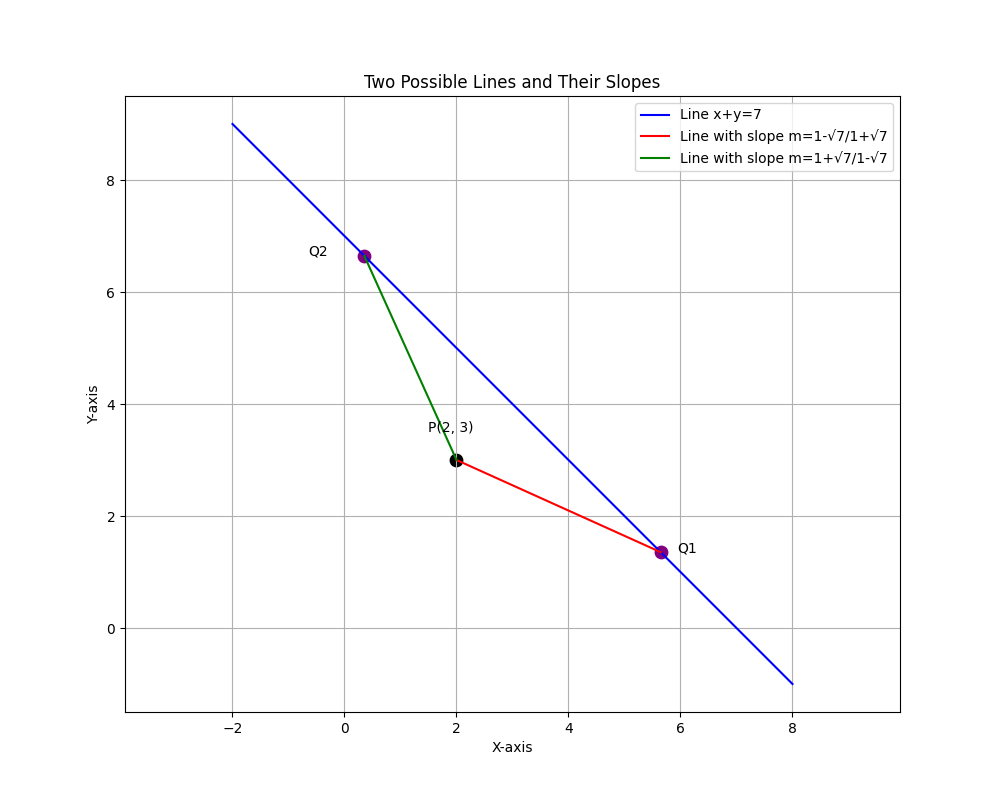
\includegraphics[width=0.7\columnwidth]{figs/fig1.png}
	\caption{}
   \label{}
\end{figure}
\end{frame}

\section{C Code}
\begin{frame}[fragile]
\frametitle{C Code}
\begin{lstlisting}[language=C]
#include <math.h>
void calculate_slope_data(double* out_data) {
    double px = 2.0, py = 3.0;
    double a = 1.0, b = -6.0, c = 2.0;
    double discriminant = sqrt(b*b - 4*a*c);
    
    double q1_x = (-b + discriminant) / (2 * a); // 3 + sqrt(7)
    double q2_x = (-b - discriminant) / (2 * a); // 3 - sqrt(7)

    double q1_y = 7 - q1_x;  
    double q2_y = 7 - q2_x;  
    
    double slope1 = (q1_y - py) / (q1_x - px);
    double slope2 = (q2_y - py) / (q2_x - px);
    out_data[0] = px;      out_data[1] = py;
    out_data[2] = q1_x;    out_data[3] = q1_y;
    out_data[4] = q2_x;    out_data[5] = q2_y;
    out_data[6] = slope1;  out_data[7] = slope2;
}
    \end{lstlisting}
\end{frame}
\section{Python Code}
\begin{frame}[fragile]
\frametitle{Python Code for Calling}
\begin{lstlisting}[language=Python]
import ctypes
import numpy as np

def get_data_from_c():
    lib = ctypes.CDLL('./code.so')
    
    double_array_8 = ctypes.c_double * 8
    lib.calculate_slope_data.argtypes = [ctypes.POINTER(ctypes.c_double)]
    out_data_c = double_array_8()
    lib.calculate_slope_data(out_data_c)
    all_data = np.array(out_data_c)
    # Unpack the data
    point_p = all_data[0:2]
    point_q1 = all_data[2:4]
    point_q2 = all_data[4:6]
    slopes = all_data[6:8]
    
    return point_p, point_q1, point_q2, slopes
\end{lstlisting}
\end{frame}
\begin{frame}[fragile]
\frametitle{Python Code for Plotting}
\begin{lstlisting}[language=Python]
#Code by GVV Sharma
#September 12, 2023
#Revised July 21, 2024
#released under GNU GPL
import sys                                          #for path to external scripts
sys.path.insert(0, '/workspaces/urban-potato/matgeo/codes/CoordGeo/') 
import numpy as np
import matplotlib.pyplot as plt

from call import get_data_from_c

# Get the points and slopes from the C library
P, Q1, Q2, slopes = get_data_from_c()
slope1, slope2 = slopes
\end{lstlisting}
\end{frame}

\begin{frame}[fragile]
\frametitle{Python Code for Plotting}
\begin{lstlisting}[language=Python]
print(f"The two possible slopes are: {slope1:.4f} and {slope2:.4f}")
x_line_given = np.array([-2, 8])
y_line_given = 7 - x_line_given

# Create points for the two possible solution lines
x_line_1 = np.array([P[0], Q1[0]])
y_line_1 = np.array([P[1], Q1[1]])
x_line_2 = np.array([P[0], Q2[0]])
y_line_2 = np.array([P[1], Q2[1]])

fig, ax = plt.subplots(figsize=(10, 8))

ax.plot(x_line_given, y_line_given, 'b-', label='Line x+y=7')
ax.plot(x_line_1, y_line_1, 'r-', label=f'Line with slope m={slope1:.2f}')
ax.plot(x_line_2, y_line_2, 'g-', label=f'Line with slope m={slope2:.2f}')
\end{lstlisting}
\end{frame}

\begin{frame}[fragile]
\frametitle{Python Code for Plotting}
\begin{lstlisting}[language=Python] 
ax.scatter(P[0], P[1], color='black', s=80)
ax.scatter(Q1[0], Q1[1], color='purple', s=80)
ax.scatter(Q2[0], Q2[1], color='purple', s=80)

ax.text(P[0] - 0.5, P[1] + 0.5, f'P({P[0]:.0f}, {P[1]:.0f})')
ax.text(Q1[0] + 0.3, Q1[1], 'Q1')
ax.text(Q2[0] - 1.0, Q2[1], 'Q2')

ax.set_title('Two Possible Lines and Their Slopes')
ax.set_xlabel('X-axis')
ax.set_ylabel('Y-axis')

ax.grid(True)
ax.axis('equal')
ax.legend()
plt.show()
plt.savefig('../figs/fig1.png')
\end{lstlisting}
\end{frame}

\end{document}
